%\section{Problems}
\begin{problem}

Consider a tight binding Hamiltonian with nearest-neighbor hopping on a general two dimensional Bravais lattice with $N$ lattice points, in contact with a particle reservoir. The chemical potential of the system is denoted $\mu$. The nearest-neighbor hopping element is given by $t$. The Hamiltonian is given by 
\begin{eqnarray}
	H = - t \sum_{\langle i,j \rangle, \sigma} c^{\dagger}_{i,\sigma} c_{j,\sigma} - \mu   \sum_{ i, \sigma} c^{\dagger}_{i,\sigma} c_{i,\sigma} \nonumber 
\end{eqnarray}
Here, $(c^{\dagger}_{i,\sigma}, c_{i,\sigma})$ create and destroy particles in spin-state $\sigma$ on site $i$. 
Introduce Fourier-transformed operators 
\begin{eqnarray}
	c^{\dagger}_{{\bf k},\sigma} & = & \frac{1}{\sqrt{N}} \sum_{i} c^{\dagger}_{i,\sigma} ~ \e^{-i {\bf k} \cdot {\bf r}_i} \nonumber  \\
	c_{{\bf k},\sigma} & = & \frac{1}{\sqrt{N}} \sum_{i} c_{i,\sigma} ~ \e^{i {\bf k} \cdot {\bf r}_i} \nonumber
\end{eqnarray}
where ${\bf r}_i$ is the position at lattice site $i$. 
\ \\
\ \\
{\bf a)} Show that Hamiltonian may be written on form
\begin{eqnarray}
	H = \sum_{{\bf k}, \sigma} E_{\bf k} ~ c^{\dagger}_{{\bf k},\sigma} c_{{\bf k},\sigma}  \nonumber 
\end{eqnarray}
and give an expression for $E_{\bf k}$ for a general two-dimensional Bravais lattice. 
\ \\
\ \\
{\bf b)} Specialize to the case of a two-dimensional square lattice, see Figure \ref{fig:squareblattice}, and give the expression for $E_{\bf k}$ in this case.
\missingfig{Missing fig: Square lattice}
%\begin{figure}[htb]
%	\centering
%	\includegraphics[width = 0.35\textwidth]{main_1.pdf}
%	\caption{Square lattice.}
%	\label{fig:squareblattice}
%\end{figure}

\newpage
\ \\
\ \\
{\bf c)} Imagine that we now consider a model on a {\it honeycomb} lattice, see Figure \ref{fig:honeycomblattice}.   Explain what the {\it principal} difference between this lattice and the square lattice is.
\missingfig{Missing fig: Honeycomb lattice}
%\begin{figure}[htb]
%	\centering
%	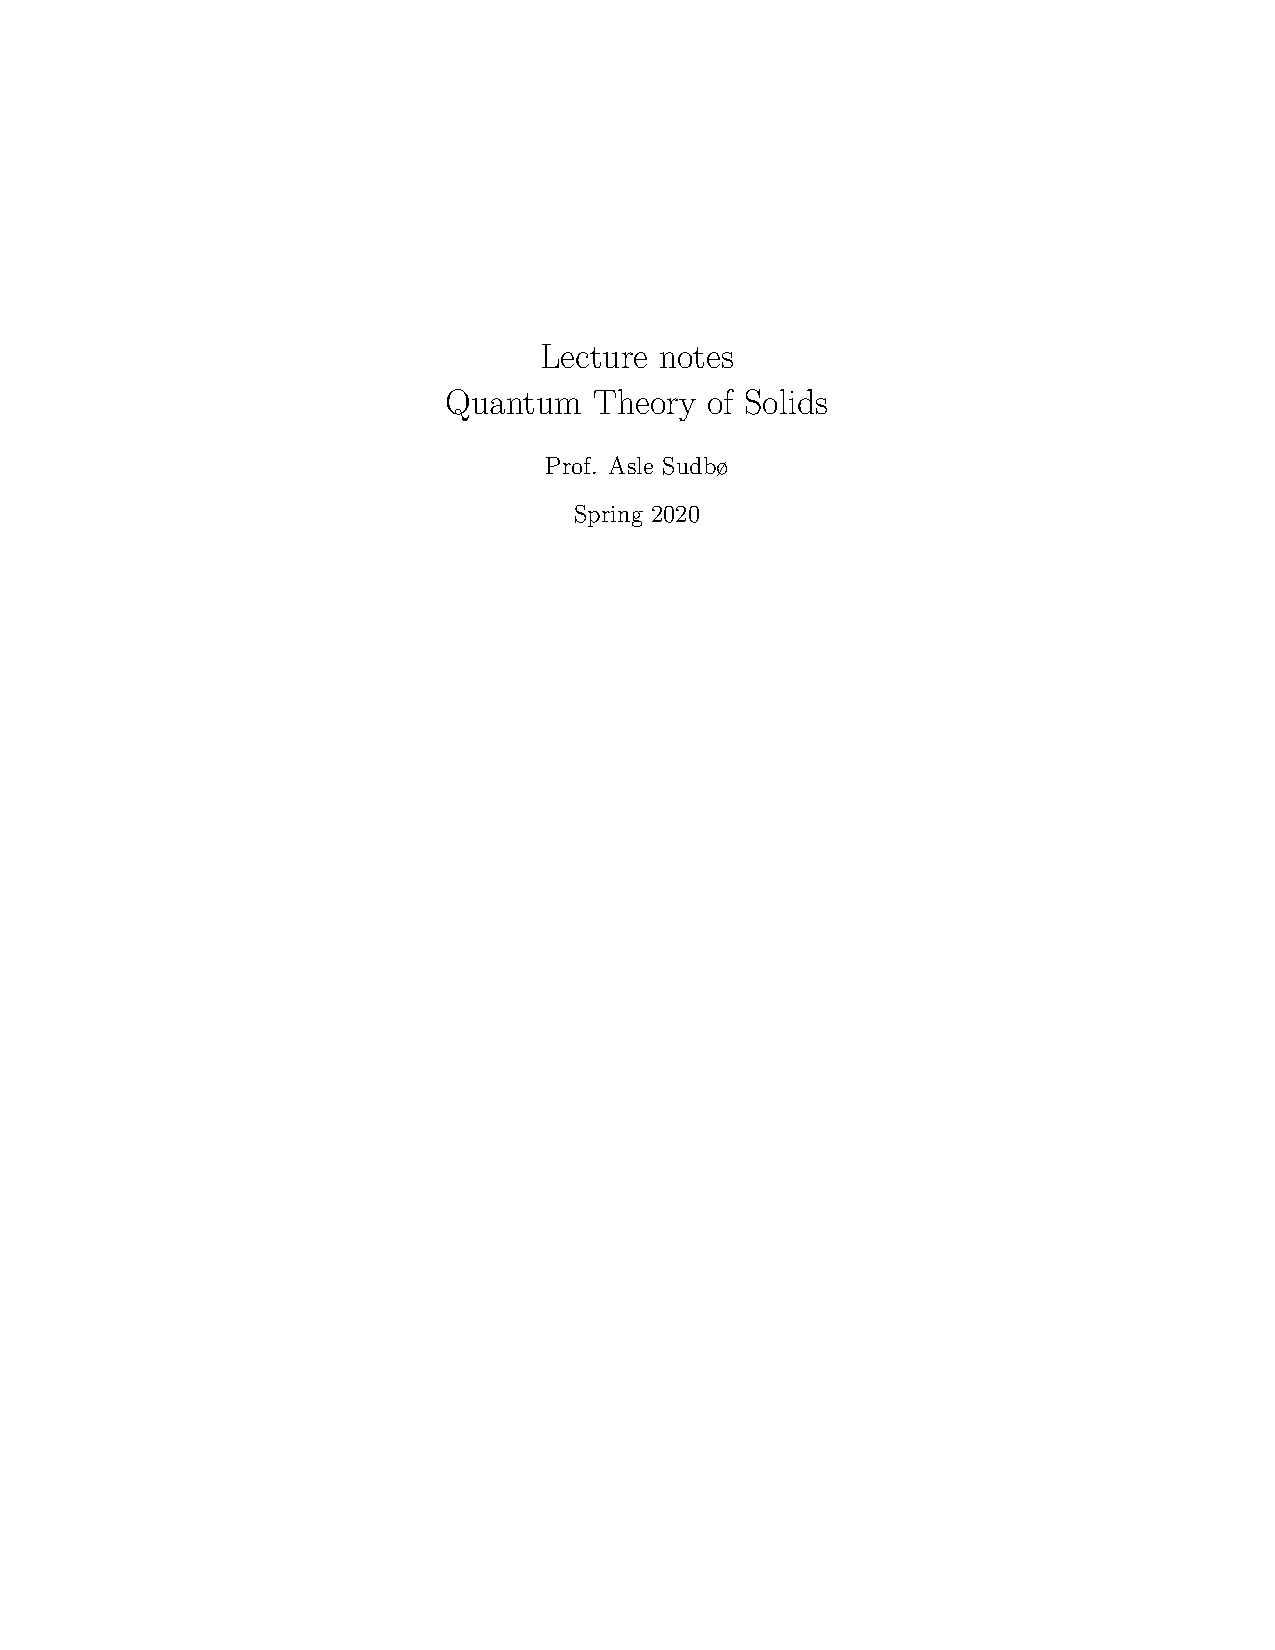
\includegraphics[width = 0.45\textwidth]{main.pdf}
%	\caption{Honeycomb lattice.}
%	\label{fig:honeycomblattice}
%\end{figure}
\ \\
\ \\
{\bf d)}  Write down a tight-binding model for this system, conidering only nearets neighbor interactions, and find $E_{\bf k}$. (Hint: You need to introduce two distinct types of fermions, one type for the red atoms and one type for the blue atoms). 
\end{problem}

\begin{problem}
Consider a tight-binding model in a uniform external magnetic field $h$ directed along the z-direction.
The Hamiltonian is given by 
\begin{eqnarray}
	H = - t \sum_{\langle i,j \rangle, \sigma} c^{\dagger}_{i,\sigma} c_{j,\sigma} - \mu   \sum_{ i, \sigma} c^{\dagger}_{i,\sigma} c_{i,\sigma}
	- h \sum_{i, \sigma} \sigma c^{\dagger}_{i \sigma}  c_{i \sigma}  
	\nonumber 
\end{eqnarray}
in the same notation as in Problem 1. The last term is the second-quantized version of the Zeeman-term 
$- {\bf h} \cdot {\bf S} = - h \sum_i S_{i z} = - h \sum_{i} \left[ c^{\dagger}_{i,\uparrow} c_{j,\uparrow}- c^{\dagger}_{i,\downarrow} c_{j,\downarrow} \right] =-  h \sum_{i, \sigma} \sigma c^{\dagger}_{i \sigma}  c_{i \sigma}.$
\ \\
\ \\
{\bf a)} Introduce the same Fourier-transform as in Problem 1, and show that the Hamiltonian may be written on the form
\begin{eqnarray}
	H = \sum_{{\bf k},\sigma} ~ E_{\bf k, \sigma} ~ c^{\dagger}_{{\bf k},\sigma} c_{{\bf k},\sigma}  \nonumber 
\end{eqnarray}
and give an expression for $E_{{\bf k},\sigma}$ for a general two-dimensional Bravais lattice. 
\ \\
\ \\
{\bf b)}  Consider instead  another variant of the tight-binding model, now in the absence of a magnetic field, but with a spin-dependent hopping matrix element. (In lectures Week 4, we discuss what the origin of such spin-dependent hopping could be). The Hamiltonian is given by, with a general spin-dependent hopping matrix element $ t^{\sigma \sigma^{\prime}}_{ij}$
\begin{eqnarray}
	H = -  \sum_{\langle i,j \rangle, \sigma, \sigma^{\prime}} t^{\sigma \sigma^{\prime}}_{ij}c^{\dagger}_{i,\sigma^{\prime}} c_{j,\sigma} - \mu   \sum_{ i, \sigma} c^{\dagger}_{i,\sigma} c_{i,\sigma}
	\nonumber 
\end{eqnarray}
Consider a special case $ t^{\sigma \sigma^{\prime}}_{ij} = t^{\sigma \sigma}_{ij} \delta_{\sigma,\sigma^{\prime}}$, with 
$t_{ij}^{\uparrow \uparrow} \neq t_{ij}^{\downarrow \downarrow}$.  Introduce the same Fourier-transform as in Problem 1, and show that the Hamiltonian may be written on the form
\begin{eqnarray}
	H = \sum_{{\bf k},\sigma} ~ E_{\bf k, \sigma} ~ c^{\dagger}_{{\bf k},\sigma} c_{{\bf k},\sigma}  \nonumber 
\end{eqnarray}
and give an expression for $E_{{\bf k},\sigma}$ for a general two-dimensional Bravais lattice. 
\ \\
\ \\
{\bf c)} Compare with the results in Problem 2 {\bf a)}, and show that this sort of spin-dependent hopping may be interpreted as particles moving in  a {\bf k}-dependent external magnetic field along the $z$-axis.  
\end{problem}
